\section{Versuchsbeschreibung}
\label{section:Versuchsbeschreibung}
%
%In diesem Versuch wird eine Peltonturbine und die dazugehörige hydraulische Anlage vermessen.
%Den benötigten Wasserdruck erzeugt eine am Boden des Aufbaus befindliche Pumpe welche über einen Kugelhahn geregelt werden kann.
%Von der Pumpe aus steigt das Wasser senkrecht auf und passiert dabei die erste Messstelle für den Wasserdruck.
%Danach knickt die Leitung um 90° ab und verläuft waagerecht. Auf der Waagerechten wird zunächst der Volumenstrom und dann erneut der Wasserdruck gemessen.\\
%Nach der Druckmessung knickt die leitung erneut um 90° ab und verläuft nun nach unten. Im Knick der Leitung befindet sich der Hahn zur Kontrolle der Düse.
%Die Düse komprimiert dann den Wasserstrahl auf die Schaufeln der Peltonturbine welche sich über einem Wasserbecken befindet und in einem Metallgehäuse ist.\\
%An die Drehachse der Peltonturbine ist ein Synchrongenerator angeschlossen, dieser ist an einem (Hebel-)Arm befestigt und mit einem Sensor zur Messung der Kraftbelastung versehen.
%An den Synchrongenerator ist wiederrum eine Schalttafel angeschlossen, welche die Einstellung und Messung des Erregerstroms ermöglicht, sowie die Einstellung des Lastwiderstandes.\\
%An diese Schalttafel werden zusätzlich 2 Multimeter angeschlossen mit welchen die Leiterspannung und der Phasenstrom gemesssen wird.
Der Versuchsaufbau besteht aus einem Wasserkreislauf angetrieben durch eine Pumpe, mit der Peltonturbine als Herzstück des Versuches.\\
Wie in \autoref{fig:Aufbau_Stillstand} zu sehen verläuft das Rohrsystem in Form eines umgedrehtens U.
Von der Pumpe aus durchläuft das Wasser unterschiedliche Messeinrichtungen und wird mittels einer Düse auf die Schaufeln der Peltonturbine komprimiert.\\
%
\begin{figure}[!ht]
    \centering
    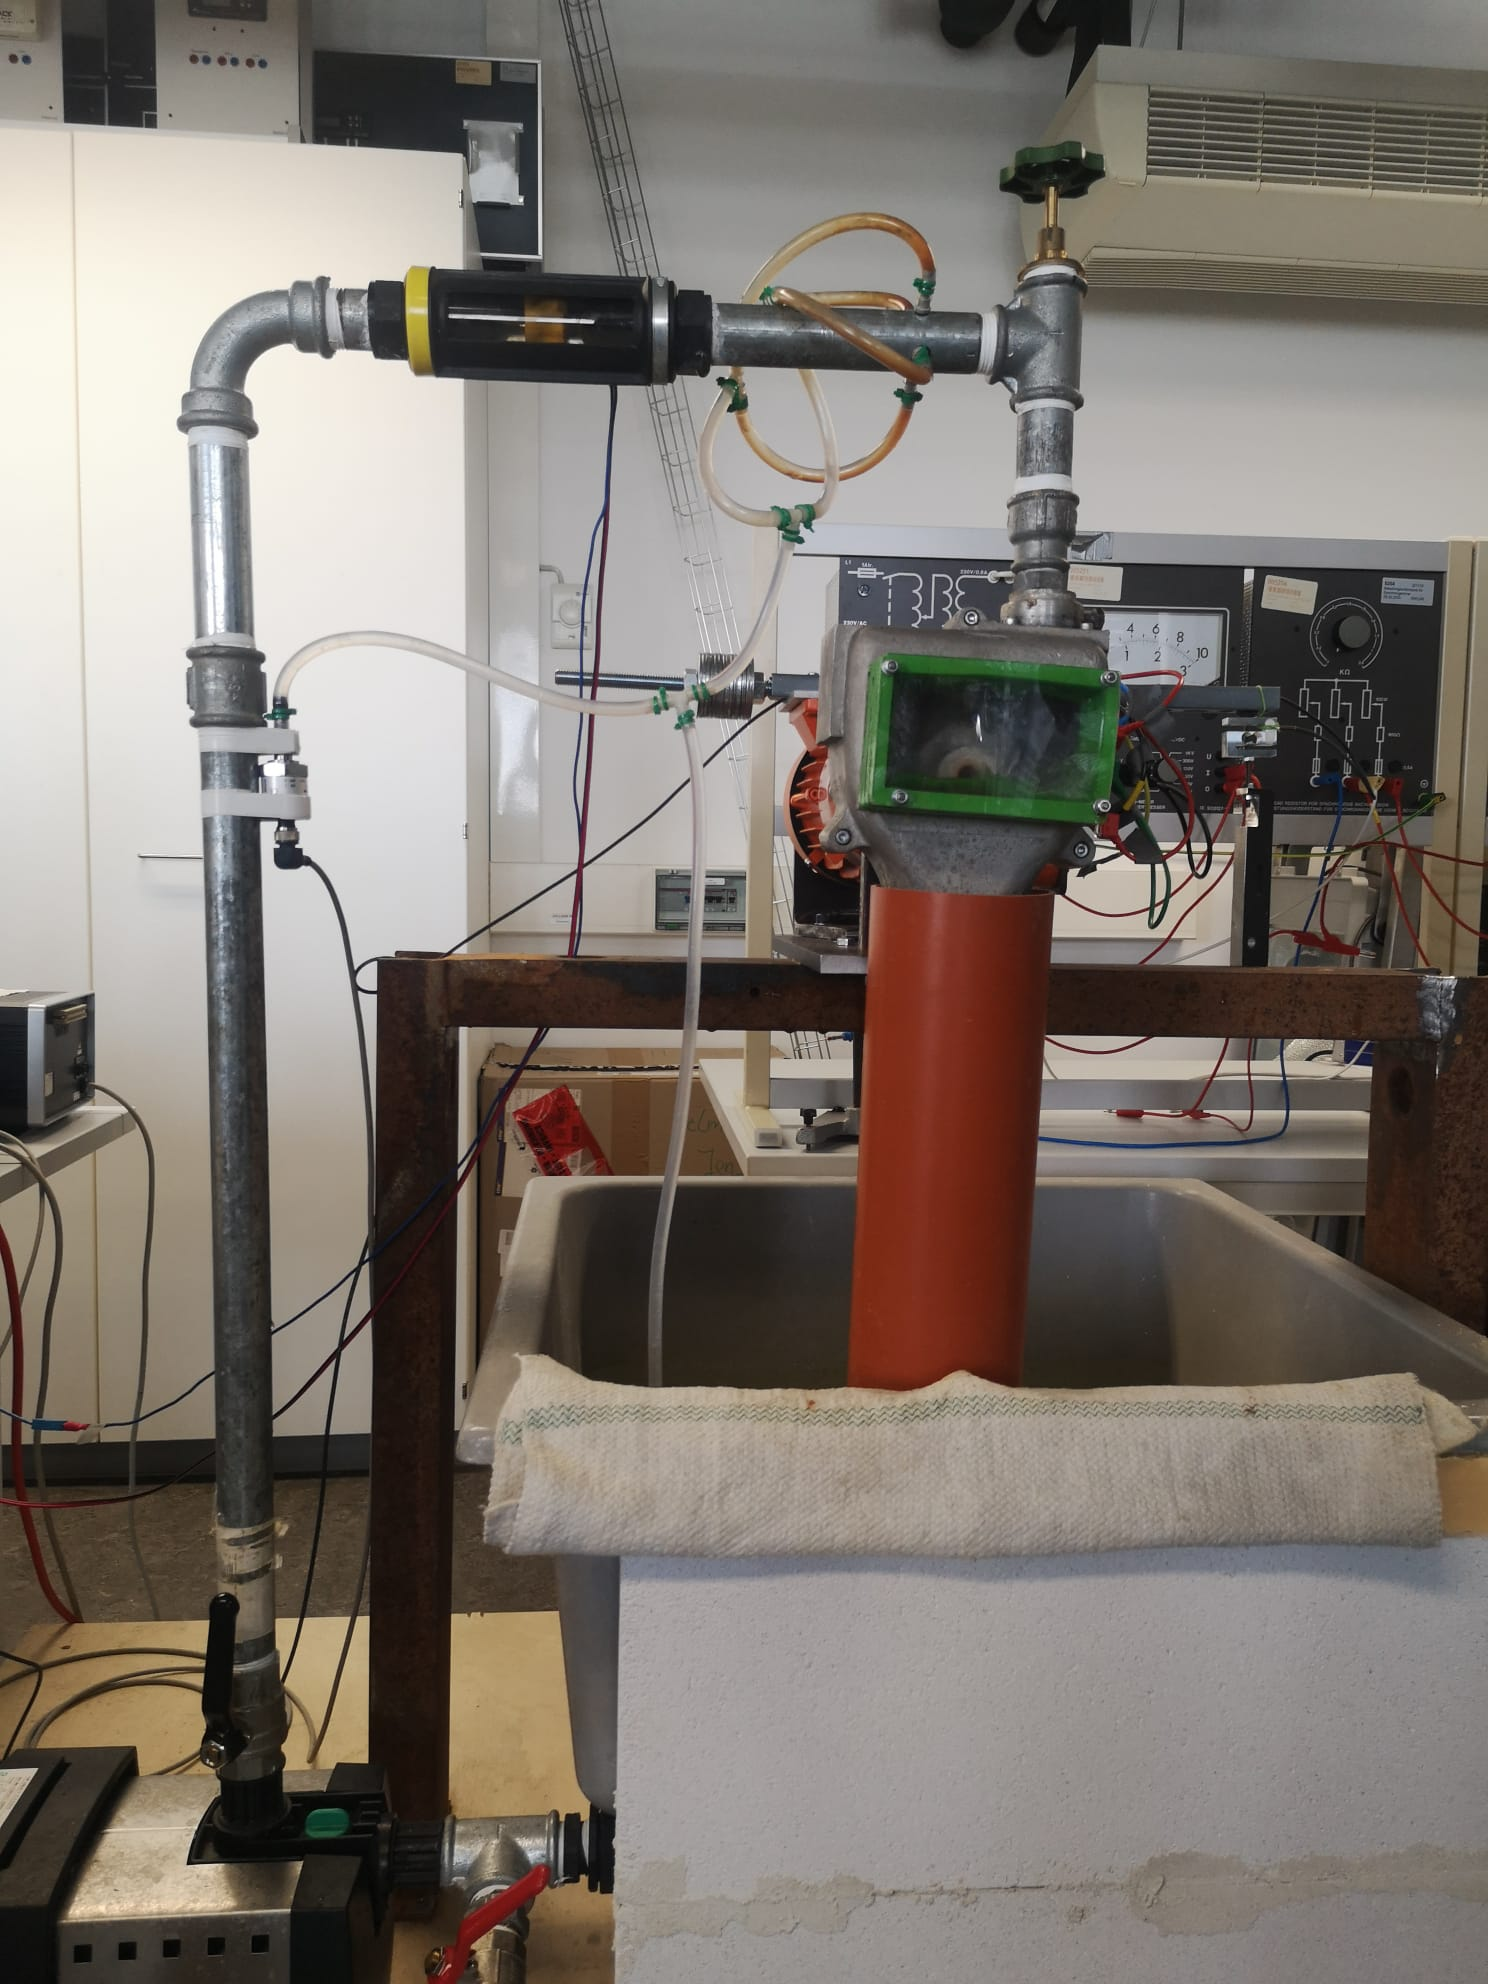
\includegraphics[width=0.5\textwidth]{Abbildungen/Aufbau Pelton.jpeg}
    \caption{Versuchsaufbau im Stillstand}
    \label{fig:Aufbau_Stillstand}
\end{figure}
\begin{figure}[!ht]
    \centering
    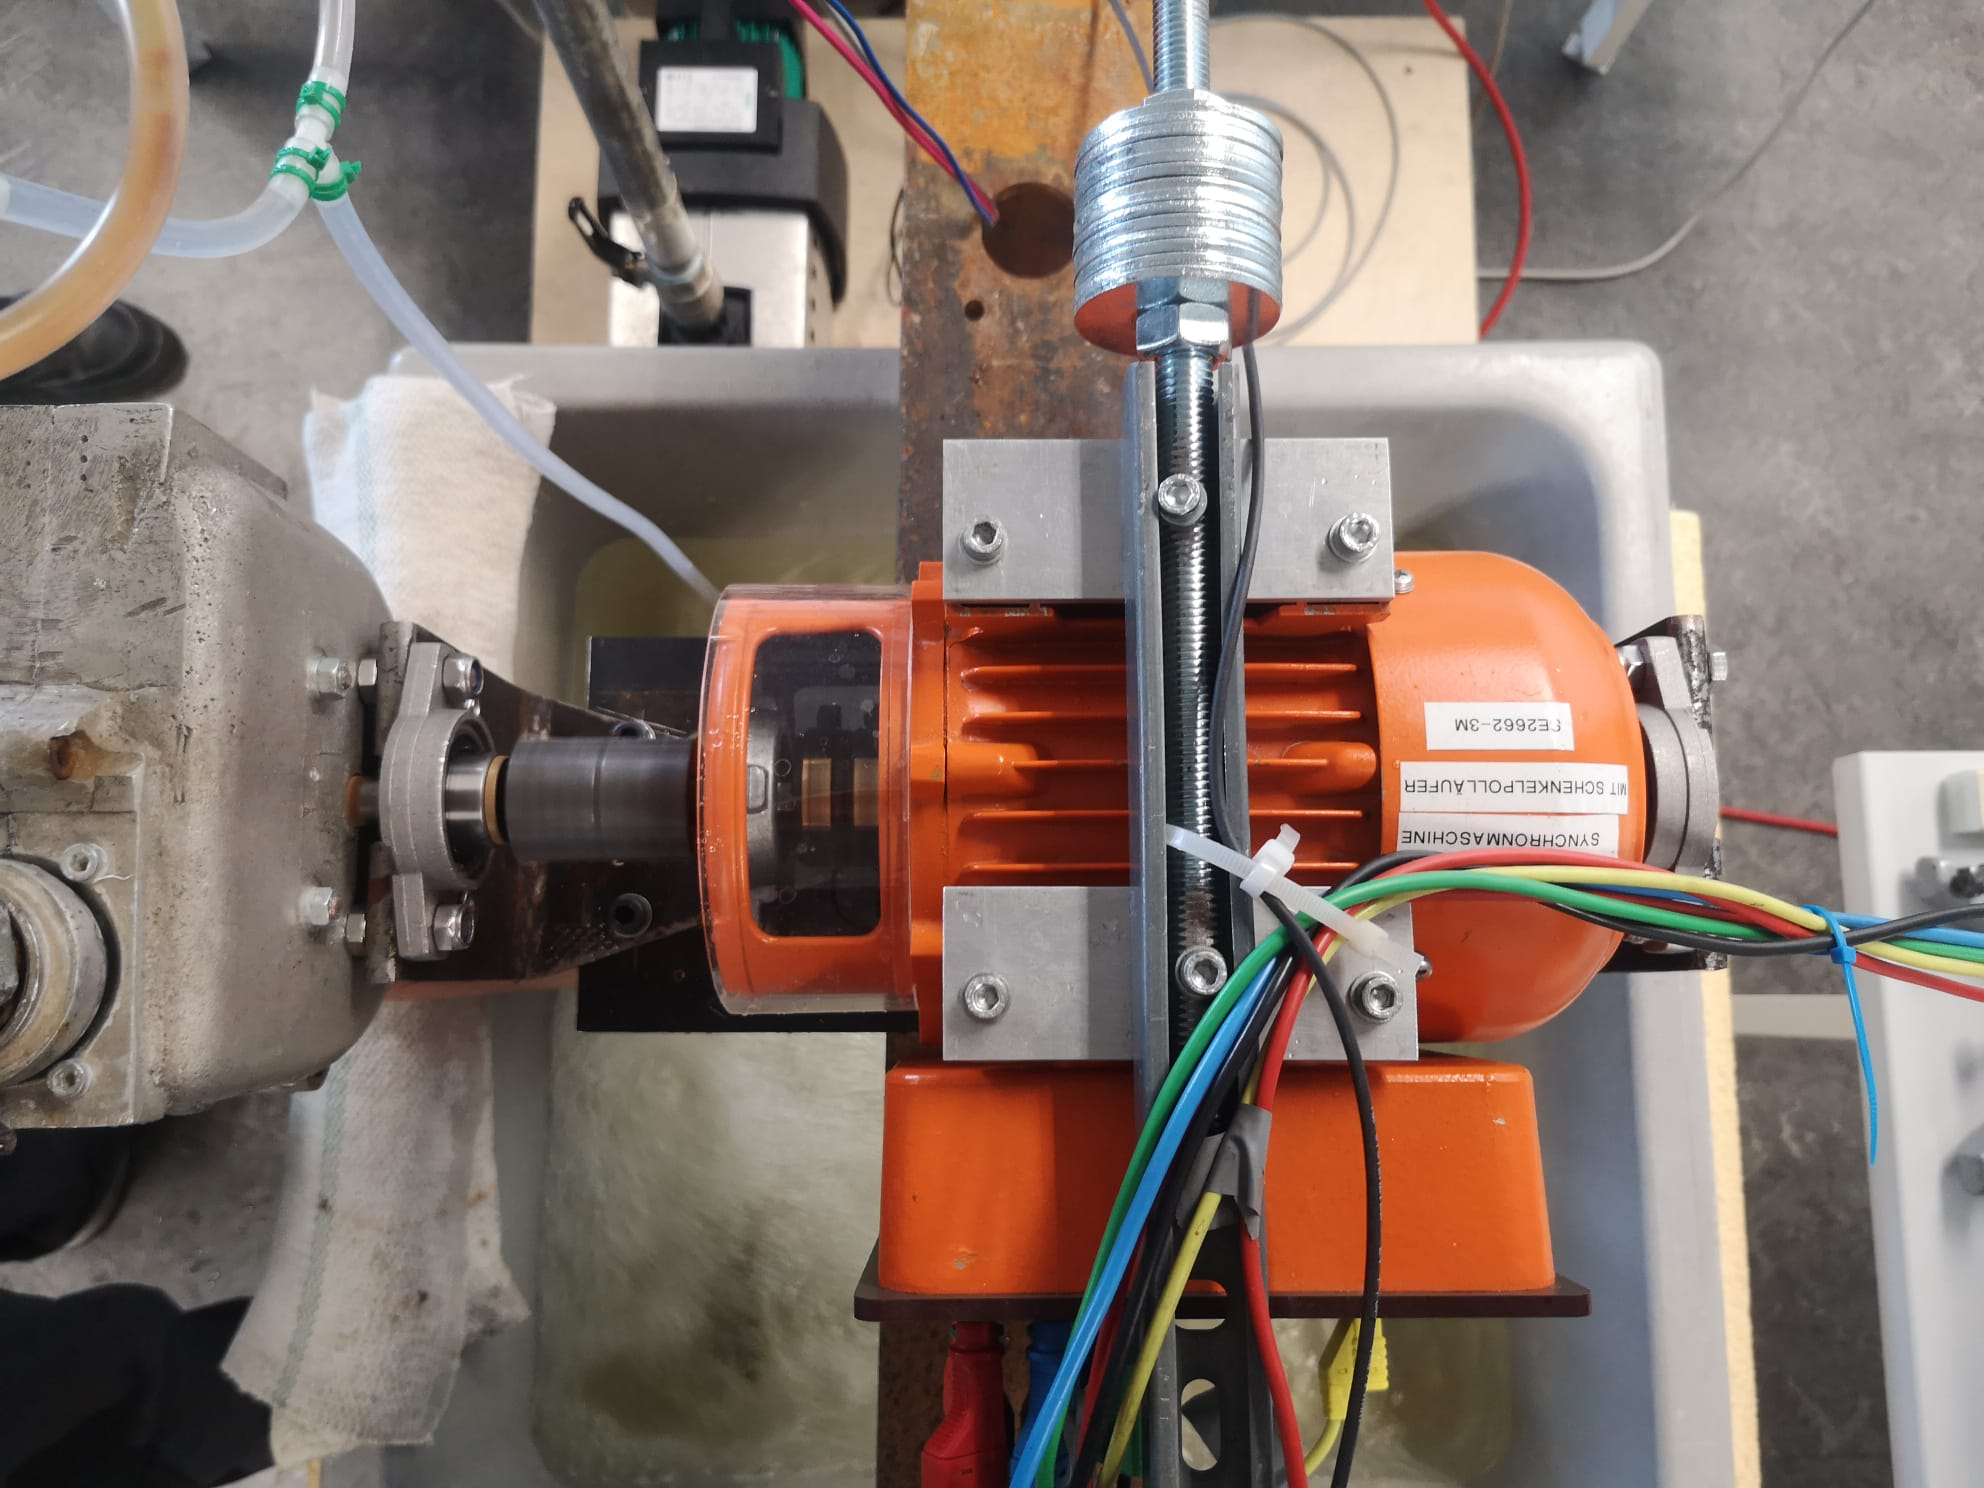
\includegraphics[width=0.5\textwidth]{Abbildungen/Generator.jpeg}
    \caption{Synchrongenerator}
    \label{fig:Synchrongenerator}
\end{figure}
\begin{figure}[H]
	\centering
	\begin{minipage}{0.49\textwidth}
		\centering
		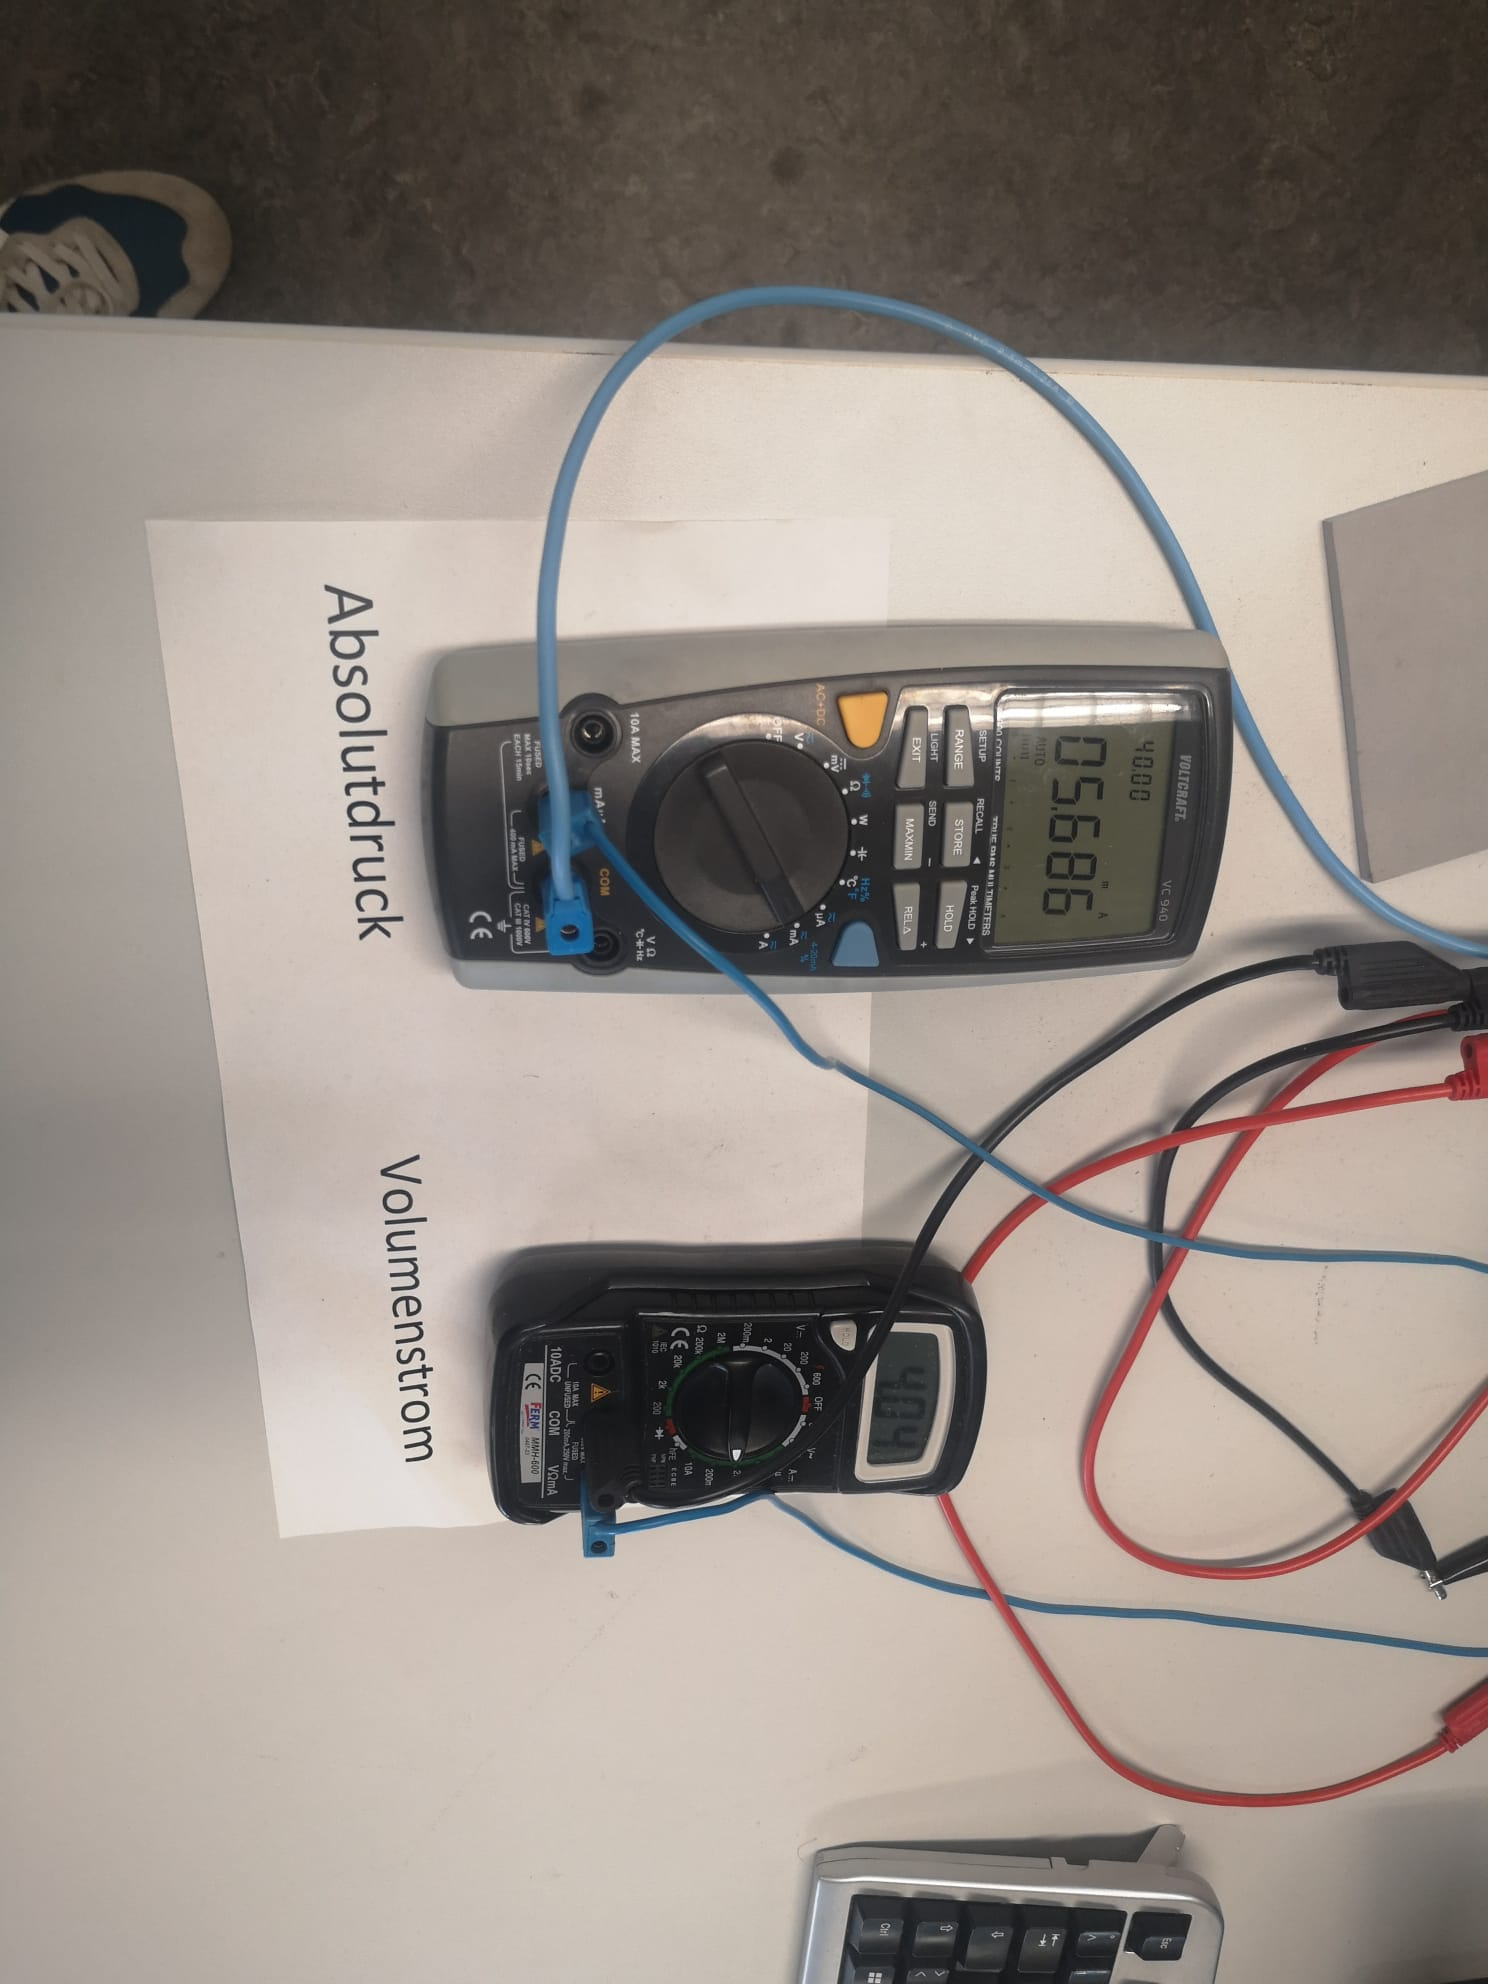
\includegraphics[width=0.7\textwidth,angle=90]{Abbildungen/Druck- & Volumenstrom-Messung.jpeg}
		\caption{Druck- und Volumenstrom-Messung}	
		\label{fig:D-V-Messung}
	\end{minipage}
	\hfill
\begin{minipage}{0.49\textwidth}
	\centering
	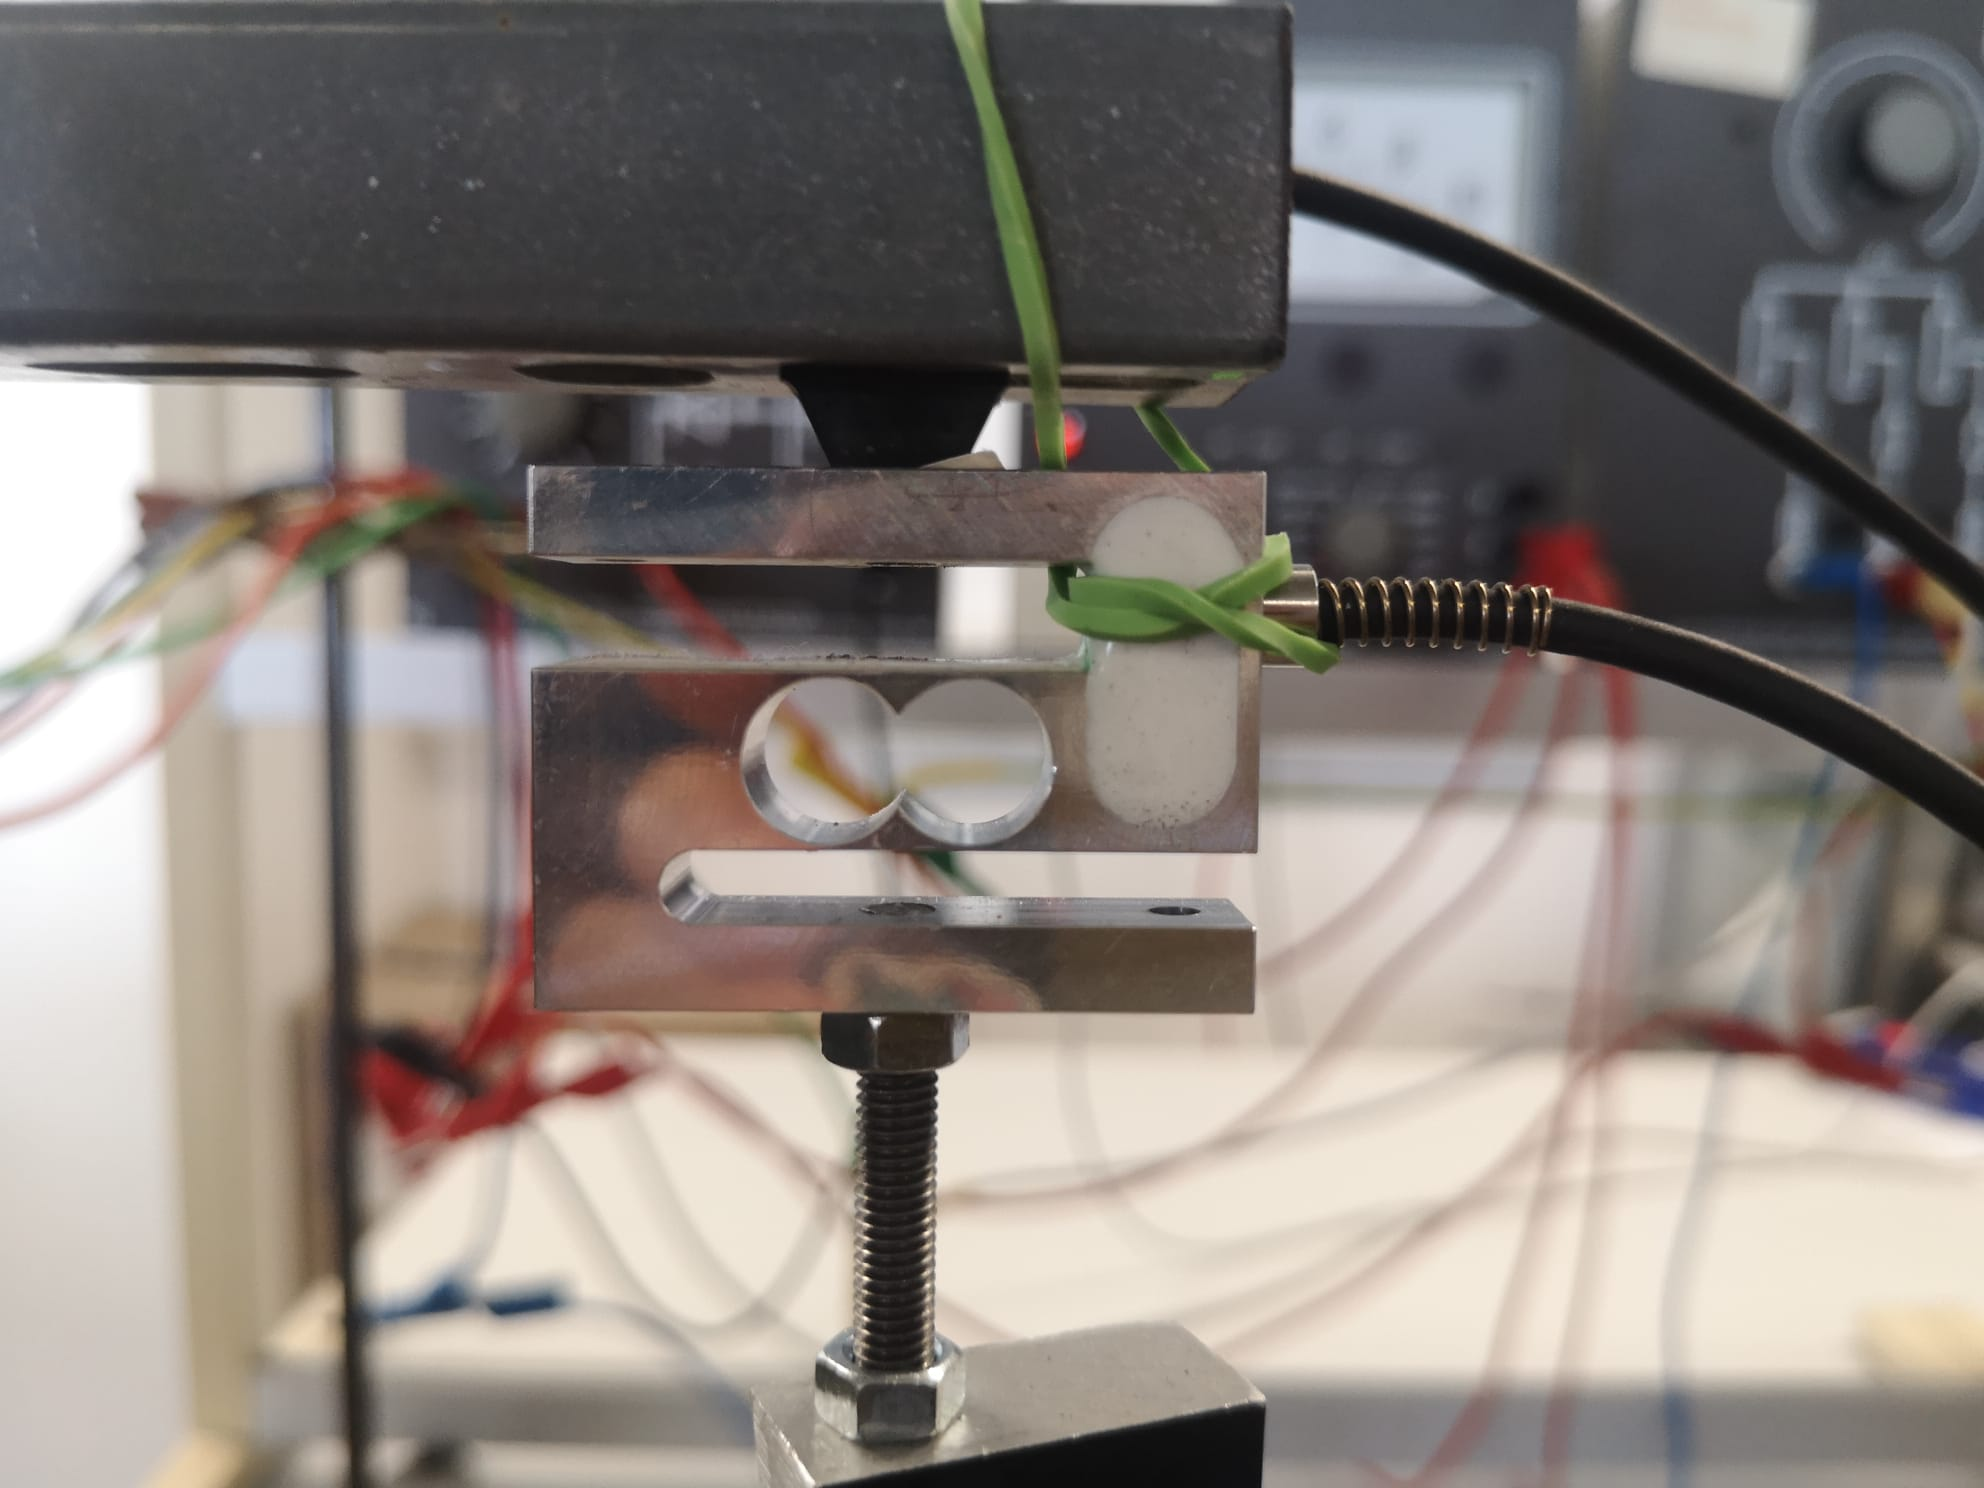
\includegraphics[width=1\textwidth]{Abbildungen/Kraftsensor.jpeg}
	\caption{Kraftsensor KD40S}
	\label{fig:KD40S}
\end{minipage}
\end{figure}
\begin{figure}[!ht]
    \centering
    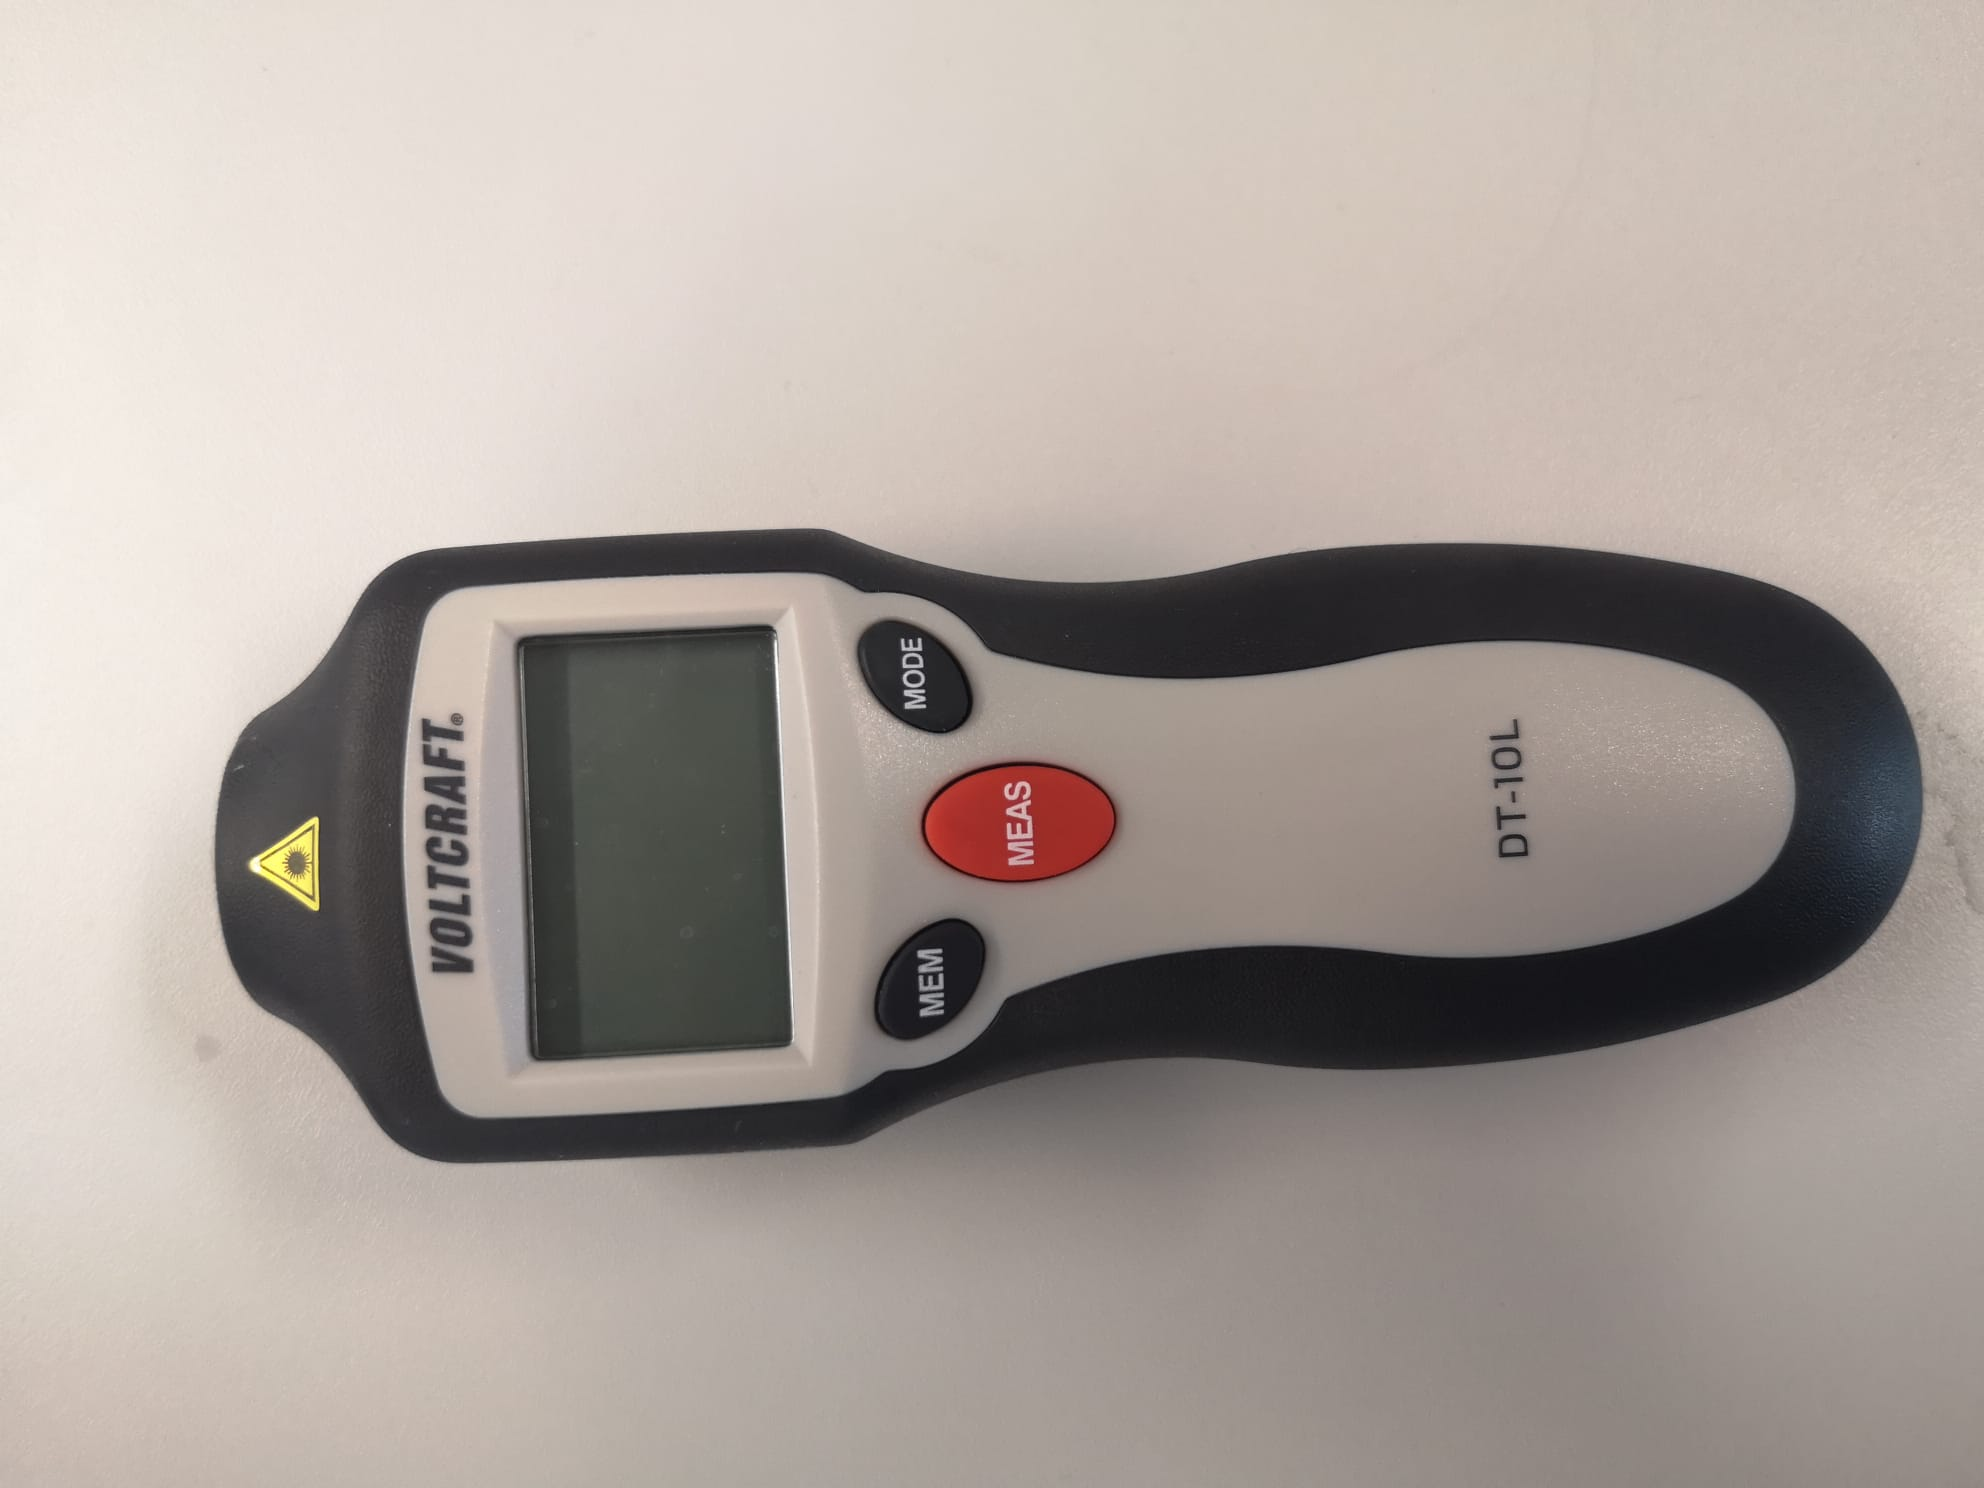
\includegraphics[width=0.5\textwidth]{Abbildungen/Drehzahlmesser 1.jpeg}
    \caption{Drehzahlmesser DT-10L}
    \label{fig:DT-10L}
\end{figure}
\begin{figure}[!ht]
    \centering
    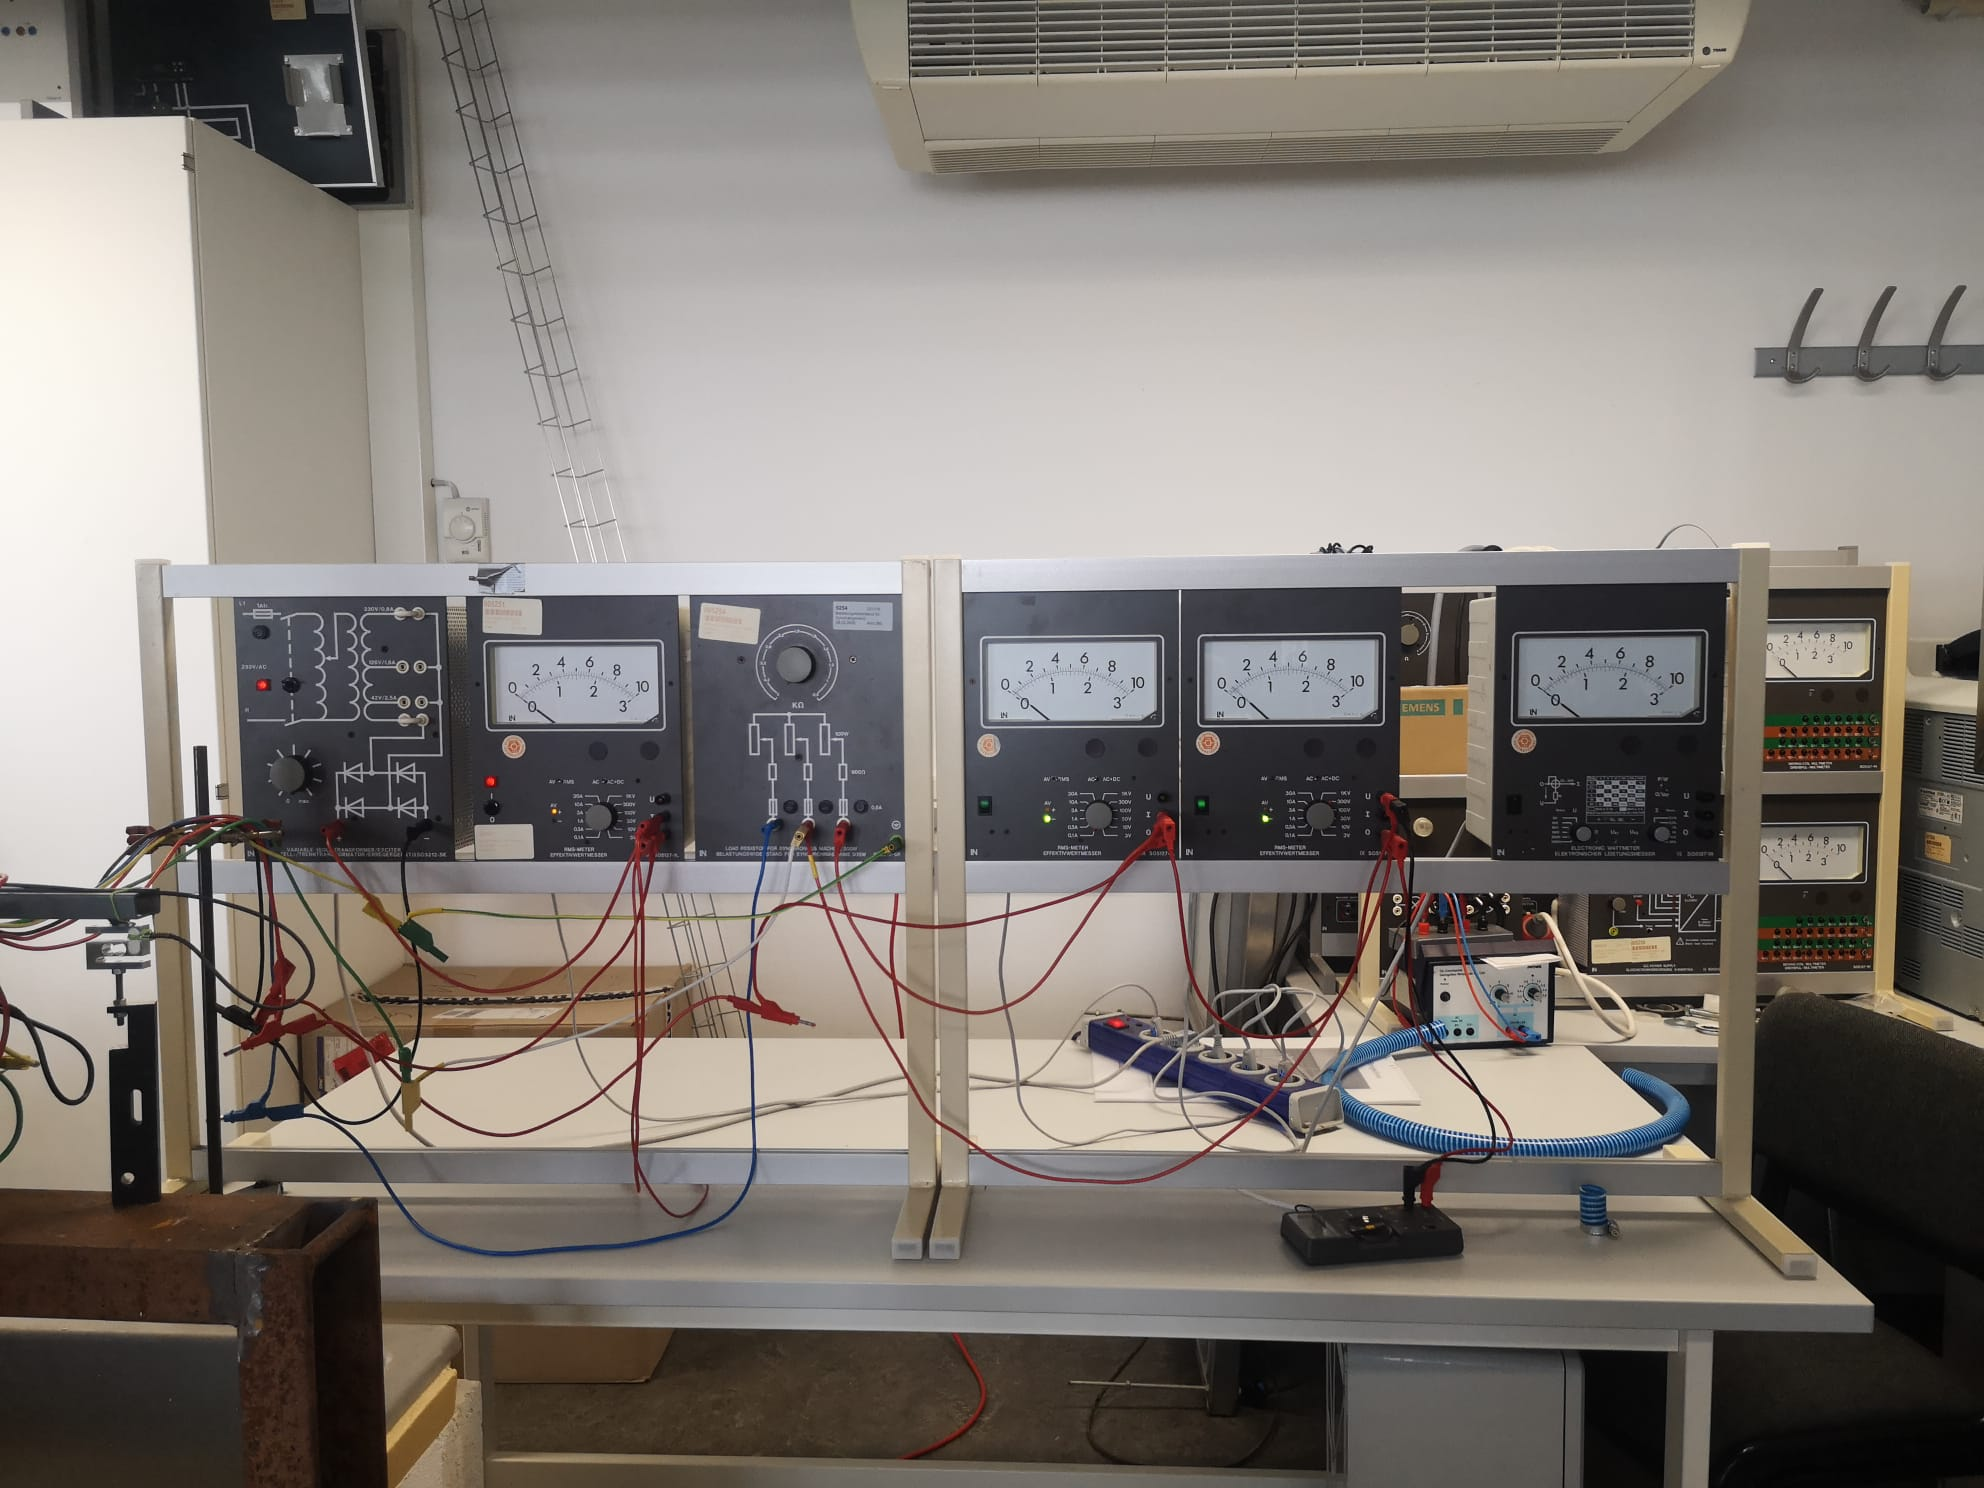
\includegraphics[width=0.5\textwidth]{Abbildungen/Schalttafel.jpeg}
    \caption{Schalttafel}
    \label{fig:Schalttafel}
\end{figure}